\begin{flushright} {\tiny {\color{gray} (tikz\_macro2.tex)}} \end{flushright}
%~~~~~~~~~~~~~~~~~~~~~~~~~~~~~~~~~~~~~~~~~~~~~~~~~~~~~~~~~~~~~~~~~~~~~~~~~~~~~~~~~~~~~~~~~~~~~~~~~~


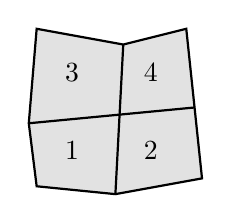
\begin{tikzpicture}
\draw[thick,fill=gray!23] (0,0)--(1,-0.1)--(2.1,0.1)--(1.9,2)--(1.1,1.8)--(0,2)--(-0.1,0.8)--cycle;  
\draw[thick] (-0.1,0.8)--(2,1);  
\draw[thick] (1,-0.1)--(1.1,1.8);  
\node[] at (0.45,0.45) {1};
\node[] at (1.45,0.45) {2};
\node[] at (0.45,1.45) {3};
\node[] at (1.45,1.45) {4};
\end{tikzpicture}



